\chapter{Literature Review}\label{C:review}

This chapter is divided into...

\section{An Overview of Web Service Composition}

At its basic level, a Web service composition is the connection of several atomic services in different configurations in order to reach a result, given that there are multiple services offering the same functionality. They key aspect of compositions is that, in order to achieve the desired result, atomic services must all be executed in a particular order, forming a workflow of tasks. A workflow-based Web service composition approach can usually be decomposed into a series of steps, reflecting the process required to produce a solution \cite{moghaddam2014service}. These steps are shown in Figure \ref{fig:steps} and discussed below:

\begin{figure}
\centerline{
\fbox{
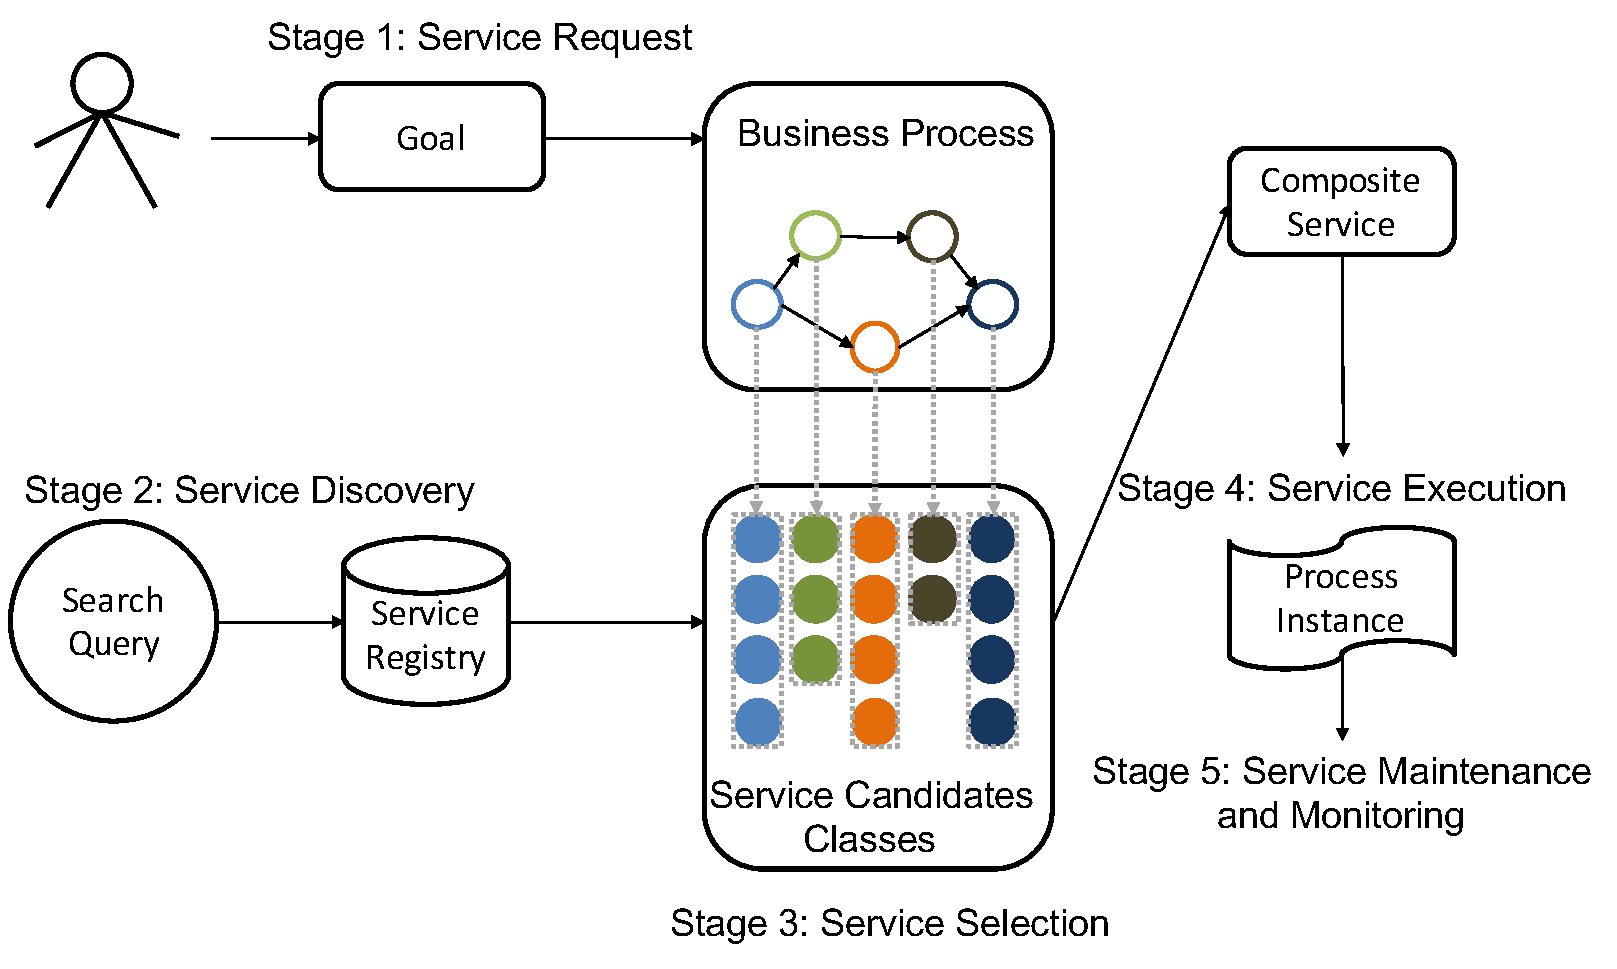
\includegraphics[width=14cm]{compositionLifecycle.pdf}
}}
\caption{Typical steps in a workflow-based automated Web service composition solution \cite{moghaddam2014service}.}
\label{fig:steps}
\end{figure}

\begin{enumerate}
 \item \textit{Goal specification:} The initial step in a Web service composition is to gather the user's goal for the solution to be produced. This is typically done through the generation of an abstract workflow that records the desired data flow and functionality details. This workflow is generated by the user and is referred to as \textit{abstract}, since it contains a series of tasks that can be accomplished by employing a number of different existing Web service implementations. In addition to this workflow, the QoS requirements are determined based on the user's preferences.
 \item \textit{Service discovery:} Once an abstract workflow and a set of preferences have been provided, the next step is to discover candidate concrete services that are functionally and non-functionally suitable to fill the workflow slots in a service repository. The focus at this stage is to find candidates that provide the functionality required to fulfil the tasks, regardless of their quality levels.
 \item \textit{Service selection:} After pools of candidate services have been identified for each workflow slot, a technique is employed to determine which discovered services best fulfil each slot. The result of this process is the creation of a concrete Web service composition.
 \item \textit{Service execution:} The creation of the composition is followed by the execution of an instance of this composed Web service.
 \item \textit{Service maintenance and monitoring:} During execution, the created instance is constantly monitored for failures and/or changes to the composing atomic services, and corrective actions are dynamically carried out as necessary.
\end{enumerate}

It is important to draw a distinction between semi-automated and fully automated composition approaches \cite{rao2005survey}. The steps discussed above are typical of a \textbf{semi-automated approach}, where an astract workflow is provided in the goal specification stage and the composition algorithm is only required to complete the abstract slots of this workflow. In a \textbf{fully automated approach}, on the other hand, an abstract workflow is not provided during the goal specification stage, and instead is calculated at the same time that services are selected based on user preferences such as the desired overall composition inputs and outputs. Consequently, service discovery may at times be also executed in tandem with the selection stage. Fully automated approaches have been shown to be more flexible than approaches with fixed abstract workflows (i.e. semi-automated approaches) with regards to solution optimisation \cite{da2014graph}, thus they are the focus of this project. It must also be noted that this work is focused on exploring new techniques to performing service selection, but not service discovery, maintenance, and monitoring.

Besides identifying the atomic Web services most suitable to fulfilling key composition tasks, the selection process often takes additional user constraints into account. A survey of the literature in the area shows that two types of contraints are commonly taken into account. The first group comprises the creation of service compositions that are optimised according to the Quality of Service (QoS) constraints on its constituent atomic services, where QoS attributes may be thought of as features that indicate the quality of a given Web service, such as the time it requires to return a response and its financial cost of execution \cite{da2014graph}. The majority of works in this area use maximising and minimising functions for the different QoS attributes, meaning that they attempt to obtain solutions with the best possible qualities without any thresholds \cite{wang2013improved,parejo2008qos,yoo2008web,garcia2008qos,zhang2010qos,wang2012survey,moghaddam2014service,kattepur2013qos,DBLP:journals/soca/LiZDSGL13}. However, there also exist approaches focused on what may be referred to as a Service Level Agreement (SLA)-aware optimisation, which is solutions must meet certain predetermined QoS thresholds in order to be considered valid (e.g. the financial cost of each service used in a composition must not exceed 50 dollars) \cite{yoo2008web,yin2014hybrid,chen2014partial,berg2013revenue}.

The second group comprises the creation of service compositions that have multiple execution branches, indicating user preferences at runtime \cite{wang2014automated,boustil2010web,karakoc2009composing,marconi2006specifying,bertoli2009control}. For example, the output of a service \textit{A} determines which service to execute next; if the output is greater than a certain threshold, then service \textit{B} should be executed; otherwise, service \textit{C} should be executed instead. These preferences are expressed logically as conditions, and affect the workflow used to establish the connections between services rather than the individual services themselves. These two types of user constraints are discussed in more detail in subsequent Sections in this chapter.

\subsection{Web Service Composition in Practice}

The research material published on Web service composition is highly theoretical and frequently employs layers of abstractions and simplifications intended to make the problem at hand manageable. However, it is also important to investigate how these ideas fit into practice, which is the objective of this Subsection. As mentioned earlier, while significant amounts of work are being performed in the field of automated Web service composition, these approaches ultimately remain on the theoretical level due to difficulties that have not yet been fully addressed. On the one hand, a study \cite{lu2007web} has shown that the composition of services is fraught with issues. A central problem is that there are discrepancies between the concepts used by different services: the schemas used differ from each other, even if the services handle exactly the same domain. Another problem is the existence of services that produce too much data, low-quality data, or that incur too much latency. These characteristics may slow down the execution of the composition and even require human intervention, defeating automation efforts.

On the other hand, an automated framework for Web service compositions which can be applied to real services has already been proposed \cite{marconi2007automatedweb}.
The functionality of this framework was demonstrated by creating a composition that uses the Amazon Virtual Cart service, the Amazon
Book Search service and a bank's Point of Sale Web service. The authors of the framework point out that it is very challenging to find service documentation that is comprehensive enough, and that functionality details had to be identified from natural language explanations intended
for developers who are working manually. Additionally, the specification of control flow requirements must be performed manually using a logic programming language. Despite these difficulties, the evaluation of this framework shows that a composition can be found within seconds when using it as opposed to an estimated 20 hours of manual development, showing that research on Web service composition provides some immediate benefits.

These two works provide opposing views on the viability of automated Web service composition, however a more recent approach \cite{mobedpour2013user} presents the interesting middle ground of user-centered design. This systems combines manual and automated techniques, providing a browsing tool that allows users to explore the repository and gain some understanding of the offered QoS value ranges of services before having to write any QoS requirements, as users may often be unaware of what a reasonable QoS value would be for a given dataset. Users are also supported through the selection process by utilising a UI that diminishes their cognitive overload, and helps them express their requirements using a standardised language. In addition to these tools, this approach also proposes a clustering algorithm that groups service candidates according to their range of QoS values, with the objective of providing selection options when users have fuzzy (i.e. soft) requirements. The strength of this approach is that it does not undervalue human intervention in the composition process, instead providing tools that empower system users. As Web service composition always requires some degree of user involvement, at the very least when setting composition requirements, this type of approach may prove to become an increasingly popular composition solution.

\section{Single-Objective QoS-Aware Composition Approaches}\label{ECandQoS}

This section discusses composition approaches that optimise solutions according to their overall QoS. These approaches can be divided into biologically inspired methods, which use Evolutionary Computation to reach their goal, ang general optimisation approaches that do not turn to evolutionary techniques. These two groups are quite distinct, but they have the commonality of using an objective function as the guide with which to measure the quality of the candidate solutions.

\subsection{Biologically-Inspired Approaches}

Biologically-inspired Web service composition approaches rely on evolutionary computation algorithms, which implement their search strategies by drawing inspiration from nature, namely the behaviour of social animals such as bees, fish, and ants. An important distinction between these different bio-inspired approaches is in their representations of the composition problem. These varying representations are discussed throughout this Subsection, and visually summarised in figure \ref{fig:representations}. \textbf{Genetic Algorithms (GA)} are a popular choice for tackling combinatorial optimisation problems, and thus have been widely applied to the problem of Web service composition \cite{wang2012survey}. The encoding scheme for a composition is commonly done as a vector of integers, where each integer corresponds to a candidate Web service, even though some authors have attempted to use matrix representations that also include semantic information about services. A population of candidates is evolved for several generations using generic operators, typically crossover and mutation: in crossover, equivalent sections of the vectors in two distinct candidates are swapped; in mutation, a section of one candidate's crossover is modified at random in order to introduce some genetic diversity. An observed problem with the GA technique is that it tends to prematurely converge to solutions, thus preventing the exploration of further possibilities. \textbf{Particle Swarm Optimisation (PSO)} bears similarities with GA, also relying a on vector representation for candidates. However, instead of employing genetic operators to carry out the search process, PSO uses the concept of position updates to move candidate particles across the search space. As PSO may also present the problem of not fully optimising solutions (i.e. converging prematurely), hybrid approaches have been attempted to improve its efficiency and optimisation power \cite{wang2012survey}. A key limitation of both GA and PSO is in the underlying vector representation used by candidates, since it makes it very challenging to encode workflow information and thus perform any type of fully automated Web service composition.

\begin{figure}
\centerline{
\fbox{
%\includegraphics[width=14cm]{}
}}
\caption{The different problem representations employed by biologically-inspired Web service composition approaches.}
\label{fig:representations}
\end{figure}

textbf{Ant Colony Optimisation (ACO)} has also been proposed as a solution to QoS-aware Web service composition \cite{zhang2010qos}. ACO is particularly suitable to a directed acyclic graph (DAG) representation, in other words, the workflow composition representation commonly used in the field. In ACO, the Web service workflow is built to be traversed by a group of ants (agents). At each fork in the graph, the ants choose which path to follow based on probabilities that take into account the strength of the pheromones left by other ants, and also a heuristic function for that particular graph. The pheromones left by the ants are updated after all ants have toured through the graph once, with paths of higher fitness resulting in a larger pheromone increment for the edges of those paths. Meanwhile, the pheromone level of all edges gradually decreases (i.e. evaporates) after each tour of the ants. The graph representation in this technique follows the abstract workflow idea, with a pool of concrete Web services associated to each abstract Web service. Each pool of candidates is a layer that is fully connected to the layers of any following abstract services, so that an optimal path can be chosen from the edges laid out. For each concrete Web service, the heuristic factor is calculated based on its QoS values, and the fitness function also measures QoS attributes. As with GA and PSO, this representation also amounts to the idea of semi-automated Web service composition, even though in this case the encoding of workflow information leading to a fully-automated approach would seem to be trivial.

The work in \cite{zhang2010qos} applies the \textbf{Artificial Bee Colony (ABC)} algorithm to Web service composition. The ABC algorithm simulates the behaviour of bees search for food sources. The position of food corresponds to candidate solutions in the search space, encoded as a service vector, and there are three types of bees dedicated to searching: \textit{Employed bees} exploit the neighbourhood of a single food source already found; \textit{Onlooker bees} exploit the neighbourhood of different food sources depending on the dance behaviour displayed by employed bees; \textit{Scout bees} are the bees sent to random food sources after the neighbourhood they were previously exploiting does not present any food sources that are better than the original. The roles of the bees change according to the colony's needs, which is a feature unique to this algorithm. One of the issues with this approach, as pointed out by the authors, is the search space it explores. The problem with the typical search space for Web service composition is that it is organised based on the proximity of the components included into the composition. For example, given two adjacent solutions $a$ and $b$ in the search space, $a$ will only have one service that is different from all the services included in $b$. Despite being neighbours, however, the fitness values of $a$ and $b$ may be radically different, and as the optimisation occurs according to a fitness function, this means that the search space is not entirely continuous. This work modified the traditional ABC algorithm to take this problem into account, filtering the neighbourhood of each solution during the search and excluding radically different neighbours from consideration.

\textbf{Genetic Programming (GP)} is, from this project's perspective, possibly the most interesting technique for the problem of Web service composition. That is because GP, unlike the previously discussed techniques, is capable of supporting fully automated Web service composition. In GP approaches \cite{aversano2006genetic,rodriguez2010composition}, workflow constructs are typically represented as the GP tree's non-terminal tree nodes while atomic Web service are represented as the terminal nodes. In this context, workflow constructs represent the output-input connections between two services. For example, if two services are sequentially connected, so that output of service \textit{A} is used as the input of service \textit{B}, this would be represented by a sequence workflow construct having \textit{A} as the left child and \textit{B} as the right one. The initial population may be created randomly, in which case the initial compositions represented in that generation are very unlikely to be executable due to their mismatched inputs and outputs, or it may be created using an algorithm that restricts the tree structure configurations allowed in the tree to feasible solutions only. A fitness function is employed for the QoS optimisation of candidates, and the genetic operators employed for this evolutionary process are crossover, where two subtrees from two individuals are randomly selected and swapped, and mutation, where a subtree for an individual is replaced with a randomly generated substitute. One of the difficulties of tackling the problem of Web service composition using GP is that it does not intrinsically support the use of constraints \cite{craenen2001handle}, meaning that even if all candidates in a population meet the feasibility constraints, there is no guarantee that subsequent generations will maintain conformance to them. The approaches discussed above handle this problem in one of two ways: by \textit{indirect constraint handling}, where feasibility constraints are incorporated into the fitness function so that the optimal function value reflects the satisfaction of all constraints, or by \textit{direct constraint handling}, where the basic GP algorithm is adapted at the initialisation and genetic operation stages to ensure that the feasibility constraints are met. Indeed, the tree representation of an underlying workflow composition may pose difficulties whenever constraint verification is necessary.

\subsection{General Optimisation Approaches}


Don't use biologically inspired approaches. However, they are capable of producing optimised results. There are many out there, so
these are a subset only.

-> Tabu

-> ILP

-> Structural Equation Modelling

-> Algebraic expressions (? -- last paper in summary list for this section)

\textit{An Improved Artificial Bee Colony Approach to QoS-Aware Service Selection \cite{wang2013improved}}
This work applies the ABC algorithm to Web service composition. While ABC is a relatively straightforward algorithm, it requires a search space
that presents the property of \textit{optimal continuity}. This means that any given location in the search space has neighbouring locations with
similar characteristics, so fitness evaluations around the same area should result in somewhat continuous fitness values. According to the authors,
however, the Web service composition search space does not typically possess optimal continuity, which makes the employment of ABC challenging.
The paper presents a technique to create an analogous search space from the original WSC space which presents optimal continuity, thus enabling the
use of a simple ABC algorithm (without the need for modifications that are typically necessary due to the lack of this property).

The ABC algorithm simulates the behaviour of bees searching for food sources. The position of food corresponds to candidate solutions in the
search space, and there are three types of bees dedicated to searching: \textit{Employed bees} exploit the neighbourhood of a single food
source already found; \textit{Onlooker bees} exploit the neighbourhood of different food sources depending on the dance behaviour displayed by
employed bees; \textit{Scout bees} are the bees sent to random food sources after the neighbourhood they were previously exploiting does not
present any food sources that are  better than the original. The roles of the bees change according to the colony's needs, which is a feature
unique to this algorithm.

The problem with the typical search space for Web service composition is that it is organised based on the proximity of the components included
into the composition. For example, given two adjacent solutions $a$ and $b$ in the search space, $a$ will only have one service that is different
from all the services included in $b$. Despite being neighbours, however, the fitness values of $a$ and $b$ may be radically different, and as
the optimisation occurs according to a fitness function, this means that the search space does not hold the property of optimal continuity.
In order to create a search space with more desirable properties, the following must be done: when checking each neighbour $n$ of a Web service
composition candidate $c$, all atomic services that are different in $n$ and $c$ must be compared. The only true neighbours of $c$ are those
compositions $n$ where the differing services are only distinct up to a given threshold. For example, in the case of a fitness function that optimises
solutions purely based on a QoS availability measure, the difference in availability between each of the differing pairs of atomic services in $n$ and $c$
must not exceed a given threshold, say 0.1. So if the differing service in $c$ has an availability of 0.5, then the availability in the corresponding service in $n$
can only range from 0.4 to 0.7. If this requirement is not met, $n$ is not considered a real neighbour of $c$ with regards to optimal continuity.
Checking for optimal continuity can be be accomplished by using a greedy search algorithm to filter all actual neighbours from the set of possible
neighbours.

Experiments were conducted comparing ABC with the use of thresholds for optimal continuity, and ABC without the use of such thresholds. Results
show that  while the version with thresholds takes slightly longer to execute, the optimality of its solutions is almost always superior.

\textit{How To Handle Constraints with Evolutionary Algorithms \cite{craenen2001handle}}\\
This paper discusses strategies for solving problems taking constraints into account and employing evolutionary algorithms. The difficulty of
implementing this scenario is that EA techniques do not intrinsically support the use of constraints, meaning that even if all candidates in a
population meet the constraints, there is no guarantee that subsequent generations will maintain conformance to them. Even though at first one
could interpret this to mean that EAs are not suitable for problems with associated constraints, upon closer inspection one can find applications
of EA techniques to constraint satisfaction problems. This is done in one of two ways: \textit{indirect constraint handling}, where
constraints are incorporated into the fitness function so that the optimal function value reflects the satisfaction of all constraints,
or \textit{direct constraint handling}, where the chosen EA technique is adapted to ensure the constraints are met. For direct constraint handling,
modifications (with various incurring costs) may include discarding/repairing the candidates that violate constraints, employing special operators
that preserve constraints, and transformations to the search space so that all solutions are already constrained. The paper lists several categories
of evolutionary constraint satisfaction problem (CSP) solvers, including the use of modified operators that rely on heuristics to guide the transformed
parts of a candidate towards constraint satisfaction, and of a co-evolutionary approach where a population of constraints is used alongside an evolving
population of solutions (the top solution candidates are matched against a given constraint, and the fitness history for that candidate is updated according
to points showing how well they match the constraints). The question of how well EAs work for constraint solving problems when compared to
more traditional techniques is raised, but as an appropriate comparison methodology has not been fully developed at this stage no conclusions can be made
in this regard.

\textit{Tabu Search - Part I \cite{glover1989tabu}}\\
This paper presents a combinatorial optimisation strategy called Tabu search. In combinatorial optimisation, the goal is to find an optimal solution within a group
of candidates, typically in problems where exhaustive search is prohibitively expensive. The Travelling Salesman Problem (TSP) is an example of a problem that entails
combinatorial optimisation. In Tabu search, an objective function (either linear or nonlinear) is used to measure the goodness of solutions, encouraging solutions with
the least penalty (i.e. optimal solutions). Then, a range of moves that lead from one candidate solution to another is defined. For a particular candidate solution,
there is a set of moves that can be applied to it, and this is known as the neighbourhood function. One of the biggest advantages of Tabu search is that, unlike the
hill climbing technique, it can avoid being stuck at local optima when searching. The technique keeps track of a set of tabu moves, which are moves that violate a given
collection of tabu conditions. A simple Tabu search has the following steps:

\begin{enumerate}
 \item Select an initial solution and set it as the best so far. Set iteration counter \textit{k} to 0 and create an empty tabu set.
 \item If the set of potential moves from the current solution, excluding those in the tabu set, is empty, go to step 4. Otherwise, increment \textit{k} and
 select the best next move (measured using the objective function).
 \item If the next move is better than the best solution so far, update the best solution.
 \item If the chosen number of iterations has reached a limit since the best solution so far was updated, or if there are no possible non-tabu moves, stop.
 Otherwise, update the tabu set and return to step 2. A simple way of updating this set is by keeping track of the inverse moves (i.e. the moves that would
 reverse each of the moves) for a \textit{t} number of previous iterations. 
\end{enumerate}

The objective of having a tabu set is to prevent the search from reaching solutions whose best next move has already been visited before (i.e. prevent cyclic
search moves). Due to its relative simplicity and its flexibility of implementation, tabu search has a wide range of practical applications for combinatorial
optimisation problems.

\textit{QoS-Aware Services Composition using Tabu Search and Hybrid Genetic Algorithms \cite{parejo2008qos}}\\
This work applies Tabu search and a hybrid version of the Genetic Algorithm (GA) technique to QoS-aware web service composition. The composition handled by
this paper is semi-automated, so the techniques are employed for discovering concrete services that fulfil the desired abstract functionality requirements.
For the Tabu search, a move is defined as a change in one of the concrete services used as the solution, and the Tabu set is a fixed-size set of the latest
\textit{n} solutions visited. This Tabu implementation also uses an aspiration condition, which allows solutions currently in the Tabu set to be reconsidered
if they are really promising (?). For the hybrid genetic algorithm, the same basic idea of the traditional GA is applied (set candidate sizes, two-point crossover,
mutation that randomly chooses another concrete service), however a local improver is also employed. This improvement process randomly explores a percentage of
a solution's neighbourhood. These two approaches are compared with a standard GA implementation using a randomly generated dataset, and results show that the hybrid
GA approach (HGA) reaches the best overall fitness, closely followed by the Tabu approach. The drawback of these methods is that their parameters, such as the size
of the Tabu set and the percentage of solutions locally explored in HGA, must be well tuned in order to achieve good solutions.

\textit{A Web Service Composition Framework Using Integer Programming with Non-Functional Objectives and Constraints \cite{yoo2008web}}\\
This paper proposes a fully automated Web service composition approach that also takes non-functional attributes (QoS) into account when constructing the
best solution, using Integer Linear Programming (ILP). An objective function is defined for the achieving the optimal QoS values, and several other functions
are used to restrict the functionality of the solutions (i.e. restrict the search space). For linear programming, we first determine the corners of the
restricted search space (i.e. where two constraint lines meet), and then apply the objective function to each of these solutions. In linear programming, it
has been proven that one of these corner solutions is the optimal solution (provided all boundary functions are linear), so the best objective function score
indicates the final solution. An architecture for a system using ILP for performing fully automated composition is proposed, but no tests are presented.
An ILP approach is likely difficult to employ if the objective is create a composition that respects user constraints such as if-else statements (might require
the use of a nonlinear function to constrain behaviour).

\textit{QoS-Aware Semantic Service Selection: An Optimization Problem \cite{garcia2008qos}}\\
This work uses a QoS ontology as the basis for the proposal of a framework that selects services according to user preferences, representing this scenario as an optimisation problem and applying a variety of techniques to solve it. Since the ontology is represented as an XML document, XSL transformations are used in order to create the initial representation to the optimisation problem, allowing a common ontology to be used for a variety of representations. Once a user expresses his/her preferences, the framework converts this information into a set of utility functions that act as optimisation constraints, and the main optimisation function maximises/minimises the quality as required. This framework was not implemented or tested in this paper.

\textit{QoS-based Dynamic Web Service Composition with Ant Colony Optimization \cite{zhang2010qos}}\\
This paper proposes the use of a multi-objective Ant Colony Optimization algorithm for QoS-aware Web service
composition. ACO is particularly suitable to the directed acyclic graph (DAG) representation used in the field.
In ACO, a graph of components (in this case, Web services) is built to be traversed by a group of ants (agents).
At each fork in the graph, the ants choose which path to follow based on probabilities that take into account
the strength of pheromones left by other ants and also a heuristic function for that particular graph. The pheromones
left by the ants are updated after all ants have toured through the graph once, with paths of higher fitness
resulting in a larger pheromone increment for the edges of those paths (calculated using a fitness function).
Meanwhile, the pheromone level of all edges gradually decreases (evaporates) after each tour of the ants.
In this work, the ACO algorithm components are implemented in the following way:

\begin{itemize}
 \item \textit{Graph:} The graph follows the abstract workflow idea, with a pool of concrete Web services
 associated with each abstract Web service. Each pool of candidates is a layer that is fully connected to
 the layers of any following abstract services, so that an optimal path can be chosen from the edges laid
 out.
 \item \textit{Heuristics:} For each concrete Web service, the heuristic factor is the sum of its normalised
  QoS values.
 \item\textit{Fitness function:} A multi-objective approach is employed, with a vector function comprising of
 variables for response time, cost, availability and reliability. An ideal vector (with the best possible values
 for each variable) is defined, and the goodness of each solution is determined by comparing its QoS vector with
 the ideal vector.
\end{itemize}

This approach was tested using a simulated composition workflow with generated concrete atomic services with varied
QoS values. Results showed that solutions can successfully be found for all tasks with values that are close to the
known ideals for the dataset, and a comparison with a multi-objective GA approach using the same fitness function
shows that the GA approach converges faster but requires 6 times more solutions than the ACO approach, but ACO
resulted in solutions with solutions closer to the optimal. Finally, ACO is shown to smoothly scale from solutions
of size 10 all the way to solutions of size 100.

\textit{A Survey on Bio-inspired Algorithms for Web Service Composition \cite{wang2012survey}}\\
This paper discusses research endeavours on Web service composition using the following techniques:
Ant Colony Algorithm, Genetic Algorithm, and Particle Swarm Optimisation.
However, before presenting information on each of these techniques it gives an overview of how the
problem of Web service composition is represented (i.e. the models of web service composition).
The paper notes that one of the limitations of this field is that there is no standard way to compare
the performance of two different approaches, so it is difficult to tell whether one has an advantage
over the other.

\subsection{Terminology}
All systems that make use of Web services use the principle of \textit{late binding}. According to this
principle, the functional needs to be fulfilled by a given service are represented by an abstract service,
and at runtime this is replaced by a concrete instance, often based on QoS measures. A composition can be
created either using \textit{local optimisation}, when the performance of each service in the composition
must be within a specified standard, or using \textit{global optimisation}, when the performance of the
overall composition must meet a given specification.  Creating a service composition with global constraints
is regarded as an NP-hard problem. Solutions to compositions can be calculated using \textit{exhaustive}
(i.e. deterministic) methods, which are expensive and scale poorly but yield the best
composition, or \textit{approximate} (i.e. nondeterministic) methods, which are cheaper but cannot
guarantee that the best composition will be found.

\subsection{Models for Web Service Composition}
At its core, Web Service Composition can be considered a \textit{combinatorial optimisation} problem, where
the objective is to find the best subset from a finite set of elements. Apart from \textit{graphs}, other representations 
for composition problems exist. These include the \textit{Knapsack problem}, where a number of items must be
selected to be a part of a solution set in order to maximise the total positive features of the set while keeping
the negative features at a minimum, and \textit{multi-objective/multi-dimensional} optimisation, where several
different goodness functions are considered simultaneously, leading to a Pareto set of results that presents different
trade-offs for each goodness measure. In this set, no result can be considered better than any other result, and no goodness
measure can be improved in a result without reducing some of its other goodness measures.

\subsection{Ant Colony Algorithm}
This algorithm is a representation of the behaviour of ants. These ants search optimal paths between a start and
an end node in a directed acyclic graph (DAG), and leave pheromones denoting the best composition path within the
DAG (note that the actual implementation of the pheromone mechanism varies from work to work, including the use of
different pheromones for different QoS attributes). In this approach, each atomic Web service is typically represented
as a node in the graph, and the QoS constraints are typically represented as weights applied to the graph edges.
However, different graph representations have also been presenting. Persisting on local optima is a potential problem
with this technique, and its efficiency is not the highest.

\subsection{Genetic Algorithm}
Genetic algorithms are a popular choice for tackling combinatorial optimisation problems, and thus have been widely
applied to the problem of Web service composition. A common representation for atomic Web services uses integer programming,
meaning that each service is represented as an integer. More specifially, linear integer programming is typically used,
restricting all constraints and fitness functions to be linear. The encoding scheme for a composition is commonly done 
as an array of integers, but some authors have attempted to use a matrix to also include semantic information (?). Researchers
also commonly investigate QoS representations, operators and fitness function variations to be applied to GA. An observed
problem with the GA technique is that it tends to prematurely converge to solutions, thus preventing it from exploring further
possibilities.

\subsection{Particle Swarm Optimisation}
Hybrid approaches have been attempted to improve the efficiency and optimisation power of PSO alone. Additionally, some 
authors have investigated the use of a PSO that is environment-aware. PSO may present the problem of not fully optimising
solutions (premature convergence).

\section{Service Selection in Web Service Composition: A Comparative Review of Existing Approaches \cite{moghaddam2014service}}
There exist two main approaches for automated Web service composition: \textit{workflow-based approaches}
and \textit{AI planning-based approaches}. In workflow-based approaches, the idea of an abstract business process that is to be
completed with concrete services is central. AI planning-based approaches, on the other hand, do not typically require this
abstract view. Composite service selection is considered an /textit{NP-hard problem}, meaning that the solution to large problems
is not likely to be found with reasonable computation times. This is typically addressed by reducing the search space.

\subsection{Lifecycle of a Typical Workflow-based WSC Solution}
A workflow-based WSC solution involves the following steps:

\begin{enumerate}
 \item \textit{Goal specification:} The user's goal and preferences for the composition are specified. An abstract workflow is generated,
 showing details about data flow and functionality, and the QoS requirements are determined based on the user's information.
 \item \textit{Service discovery:} Candidate concrete services that are functionally and non-functionally suitable to fill the slots
 in the abstract workflow are discovered in a service repository. At this stage, candidates have varying quality.
 \item \textit{Service selection:} A technique is employed to find which discovered services best fulfil each slot in the abstract
 workflow specified earlier, and a concrete Web service composition is generated.
 \item \textit{Service exection:} An instance of the concrete composition generated above is made executed.
 \item \textit{Service maintenance and monitoring:} The created instance is constantly monitored for failures and/or changes
 to the composing atomic services.
\end{enumerate}

\subsection{Optimisation-based WSC Approaches}
These approaches assume that QoS settings have already been made and are unchangeable during the period when service selection
takes places. They can also be referred to as \textit{QoS-aware} WSC approaches. One possible approach is \textit{Integer Linear
Programming}, where integers denote which services have been chosen to execute a specific task. This approach can be executed using
existing solvers, but this representation does not scale well. \textit{Genetic algorithms} are another possibility. In this case,
solutions can either be represented as a single dimension (a single execution path in the composition) or as a matrix (all execution
paths in the composition). GA is unconstrained, which may lead to solutions that are not functionally valid, therefore penalties
must be included into the fitness function employed. \textit{Constraint optimization} is another way to conceptualise WSC.
The algorithm in this technique is run according to a collection of constraints, searching for the solution that fits within
those constraints. This method is thought to be more scalable than those previously discussed. Finally, \textit{stochastic
programming} is discussed. This approach takes the non-deterministic nature of QoS attributes into account (e.g. variations in
response time, price, etc) by using a risk measure. The objective function then incorporates this measure in the creation of
a risk-aware composition. The disadvantage of this type of approach is that it does not take the dynamic nature of Web service
environments into account, assuming constancy in QoS values.

\subsection{Negotiation-based WSC Approaches}
These approaches assume that QoS settings can be modified after they have been initially set. In the context of Web service composition,
automated negotiation is used both for adjusting the details of Service Level Agreement contracts and for dynamically selecting the best
provider for particular Web services. This type of negotiation requires an organised framework, including a negotiation object (the service
with QoS attributes), a standardised protocol, and a decision-making model that implements a negotiation strategy. While this type of
approach reflects the dynamic environment of Web services, it requires a complex framework in order to be executed.

\subsection{Hybrid Approaches}
These approaches are not based purely on optimisation or negotiation, and two of them are discussed in this paper. The first one combines
\textit{optimisation and configuration}, that is, it executes an optimisation but allows users to specify ranges of values that are accepted for
each QoS attribute (as opposed to a single value). The second one combines \textit{optimisation and negotiation}, that is, if the optimisation
fails to encounter a solution with the requested QoS standards, a negotiation process is started.

\textit{GOS: A Global Optimal Selection Strategies for QoS-Aware Web Services Composition \cite{DBLP:journals/soca/LiZDSGL13}}\\
The key idea in this paper is to propose a service selection strategy that considers the future trends (forecasting) of the QoS values of the candidate
services, as opposed to relying on static snapshots of QoS values. By being able to predict the QoS trends of services, it is possible
to perform a composition that is optimal at execution time. Apart from the usual structural constraints (sequence, parallel, choice, loop,
etc) and use of normalised static QoS values, this approach also makes use of a forecast model for Web services. It is a statistical
technique called Structural Equation Modelling (SEM) that has been successfully applied to other scientific fields. One key advantage
of SEM is that it is capable of accommodating changes in the user preferences (weights) associated with each QoS attribute, and utilising
the errors associated with measuring the QoS values and measurement histories to create the forecast model. The proposed approach is tested using
two different composition algorithms enhanced with SEM, with a dataset that simulates the changes of QoS parameters over time. Results show that the prediction
model for QoS values is initially quite inaccurate, but the accuracy increases for both algorithms as days go by and a history of values is built.
The prediction error rates also decrease in the static environment (user preferences associated with QoS attributes do not change), while remaining
somewhat erratic for the dynamic environment (user preferences associated with QoS attributes vary).

\textit{QoS Composition and Analysis in Reconfigurable Web Services Choreographies \cite{kattepur2013qos}}\\
This paper studies the use of a choreography approach for QoS-aware Web service composition. As opposed to the typical techniques that
encourage a centralised composition, such as BPEL, orchestration describes how messages are passed between services without a centralised
control flow. An interesting detail about this choreographed approach is that it allows for the use of stateless and stateful services
in the same orchestration, since it defines the order in which particular service operations should be invoked. A set of algebraic expressions
and an algorithm are presented as a potential composition approach, the algorithm employing a fitness function that optimises based
on QoS attributes. This work also considers reconfigurable choreographies, which is either means that some of the services can be replaced
in the composition at runtime, or that the composition is modified in some other way.

\section{Compositions using AI Planning}

\textit{Data-Flow Requirements for Dynamic Service Composition \cite{kazhamiakin2013data}}\\
This paper proposes an approach for modelling the data flow between Web services through the use of \textit{domain objects}. For example,
the travel domain contains objects such as flight ticket, hotel reservation, etc. The key idea is to use these objects to connect the composition
needs to the services that can address them. In order to do so, authors annotate how each Web service operation relates to a given domain object.
By creating this abstraction layer of objects, it is possible to reduce the composition's dependency on implementation details for correct
execution. Now services can be thought of as having an object port proxy that leads to specific service ports. Compositions can then
be achieved by identifying the necessary domain objects for the required task. The paper goes on to show how this technique can be integrated
into existing service composition techniques, in this case AI-planning based, through the creation of a formal framework. This framework was
implemented and run with a virtual travel agency scenario. According to the authors, the implementation of such framework was not trivial, however
it successfully demonstrates that service implementations can be modified without impacting the overall composition.

\textit{Web Service Composition Integrating QoS Optimization and Redundancy Removal \cite{xia2013web}}\\
This paper argues that most QoS-aware Web service composition techniques result in solutions with redundancy, i.e. with services
that are unnecessary and could be removed from the composition without altering its functionality. To address this problem, the paper
proposes a composition technique that is still capable of optimising with regards to QoS, but also contains strategies for redundancy
removal. The approach begins by building a dependency graph of all candidate services that could be used in a composition, with layers
consisting of services with the same functionality (inputs/outputs). These layers are linked by using edges that represent how the output
of one layer may be used as the input of another. After building this graph, all layers of services that are unused (i.e. the layer's output
does not feed into any other layer's input) are removed. A path finding algorithm is used on this graph traversing forward to discover the
paths with optimal QoS values, then another algorithm traverses backward to find the least redundant path that still maintains the optimal
QoS characteristics found earlier. Experiments were carried out using the WSC dataset and comparing the composition results with two previously
published approaches, and results show that the proposed method produces solutions with a smaller number of services, meaning that redundant
services are successfully prevented from being included in the composition.

\textit{Dynamic Service Composition with Service-dependent QoS Attributes \cite{feng2013dynamic}}\\
This paper proposes a QoS-aware Web service composition that takes dependencies between services into account. For example, discounts may be granted to users
who include multiple services that are managed by the same service provider in their composition. Authors work with the notion of three types of Quality of Service
measures: default QoS (applies regardless of the preceeding services), partially dependent QoS (applies if some inputs for a service are fulfilled by outputs
of another specific service), and totally dependent QoS (applies if all inputs of a service are fulfilled by outputs of another specific service). These QoS types
are modelled in the OWL-S composition language, and are used for defining a database of the dependencies between services in a given repository. A backward,
breadth-first graph is constructed using an algorithm that takes the service dependencies into account, prioritising their inclusion whenever possible. In comparison
to state of the art techniques for QoS-aware composition, the proposed approach performs better because of its dependency detection abilities.

\textit{Specifying Data-Flow Requirements for the Automated Composition of Web Services \cite{marconi2006specifying}}\\
This paper presents a Web service composition approach that allows users to specify constraints on the data flow of the solutions
(i.e. which routes a message is allowed to take and which manipulations it can undergo). For example, consider a Web service composition
that is supposed to book a holiday for a customer using a flights, accommodation, and a map service. If it is possible to book a suitable flight
but it is not possible to book a hotel, the customer should not accept the offer. This is the type of requirement addressed by this
approach using a data flow modelling language. This is a visual language that supports the definition of inputs/outputs, forking messages,
merging messages, operations on messages, etc. By connecting these elements we obtain \textit{data nets} whose satisfiability can be clearly
verified. The composition of Web services is performed using a planning framework that is capable of interpreting and respecting the
constraints of a data net. At the time this paper was written, this approach had not yet been implemented or tested.

\textit{Control Flow Requirements for Automated Service Composition \cite{bertoli2009control}}\\
Web service compositions incur a complexity that goes beyond the simple verification of the reachability of certain outputs given certain
inputs, however many approaches do not address this fact. In this work, on the other hand, control flow requirements are also taken into
consideration, as well as the use of domain objects that are connected to service operations and can be used for defining the composition problem.
The use of domain objects is key, since it allows control flow requirements to be expressed according to them. Additionally, these objects
may evolve according to the operations performed on them. Flow constraints are defined using a formal language, and the possible states and
transitions of a given domain object are modelled using an object diagram. Similarly, it is assumed that each candidate service has a state
diagram associated with it. The service diagrams and object diagrams are then translated into state transition systems, where the composition
requirements are satisfied or not according to the states and transitions of this system. A planning framework that encodes the information
described above is employed for calculating the composition, with the composition goal being the satisfaction of user requirements. An initial
experiment, briefly reported in the paper, indicates that this approach is capable of developing a composition that handles the flow requirements
specified for a travel booking scenario. The notable characteristic of this approach is its expressiveness, since it is capable of simultaneously
handling stateful services and flow requirements while employing a fully automated composition approach.

\textit{Dynamic Service Composition \cite{khakhkhar2012dynamic}}\\
This paper presents an approach for performing dynamic service composition. As opposed to static composition, where the services that compose the solution
are selected before execution time and instantiated at runtime, in dynamic compositions the atomic services are selected at the time of execution. The advantage
of dynamic composition is that it can use the current state of the service environment as opposed to relying on information retrieved at an earlier time.
Its drawback is that it requires a composition algorithm that is fast enough to create a solution that satisfies a pending request. The problem of
service composition is often modelled as a graph in which a path is to be found, and this approach is also widely employed by researchers focusing
on dynamic composition. Forward and backward chaining approaches based on input/output matches are used for path exploration, often relying on heuristics
to encourage the exploration of the most promising paths and to reduce the number of services considered. In the approach proposed by this paper, both
forward chaining and backward chaining are employed simultaneously, with the intention of having their paths meet in the middle. By doing so, the number of
branches to be considered is greatly reduced. Experiments were performed using reduced service sets (24 services and 19 services, as shown in the paper's
appendix), and results showed that the bidirectional search implemented requires the exploration of a consistently smaller number of services when compared
to the exclusively forward and exclusively backward approaches (in these exclusive approaches, the number of services explored varied greatly according
to the dataset).

\textit{Efficient Planning for Top-K Web Service Composition \cite{deng2013efficient}}\\
This paper proposes a planning-graph approach to creating a Web service composition technique that is capable of identifying the top K solutions with regards to
overall QoS values. According to authors, AI planning is highly suitable to the domain of service composition, however many planning approaches are not efficiently
executed. A notable exception to this trend is the planning-graph method, where the search space is greatly reduced through an initial search, thus allowing the
remainder of the algorithm to focus on the relevant areas of the search space. In this work, the planning-graph approach is employed in a three-part algorithm.
In the first part, a forward search is executed from the input node aiming to find the output node, gradually filtering the services that could be used in the
composition. In the second part, the optimal local QoS of each service in the remaining graph is calculated using functions that take into consideration the QoS
of the services that could possibly feed its input, also executed from the input node towards the output. Finally, a backward search algorithm is executed to
generate the top K solutions according to local values calculated in the previous step (a threshold is provided when running this algorithm to prune out the
substandard composition options). This approach was tested using the WSC2009 dataset, and results showed that the fitness of the solutions found were equivalent
to those encountered by the winning solution at the WS-Challenge 2009. The execution time for this approach was higher than the winning solution, however this
approach finds top K solutions while the winning approach only finds the top solution.

\textit{Effective Pruning Algorithm for QoS-Aware Service Composition \cite{huang2009effective}}\\
This paper proposes an automated Web service composition approach that uses a filtering algorithm to reduce the number of services considered for the
composition, organising the remaining services as a graph according to the ways in which their inputs and outputs match. Once this graph has been determined,
a modified dynamic programming approach is applied to it in order to calculate the composition with the optimal QoS. Dynamic programming is a method
that breaks problems into smaller subproblems that are then solved, ultimately leading to the solution of the parent problem. In this case, the optimal QoS
of each atomic service in the graph is calculated, taking into account its input dependencies. At the end of this process, the overall optimal QoS values are
known and the subgraph containing the solution can be extracted by searching the graph backwards. Experiments with the WSC2009 dataset show that the algorithm
has good execution times for various dataset sizes, demonstrating its scalability. This work was extended in \cite{jiang2010qsynth}, with the presentation of a composition tool
called QSynth, and the performance of formal comparisons with other state-of-the-art approaches, also producing superior results.

\textit{QoS-aware Service Compostiion over Graphplan through Graph Reachability \cite{chen2014qos}}\\
This work combines a planning algorithm and a graph search algorithm to achieve both QoS optimisation and functional correctness in Web service compositions. The
Graphplan algorithm first builds a representation of the search space as a planning graph, then finds a solution within this graph by traversing it backwards. This
standard planning approach is modified to use Dijkstra's algorithm when performing the backwards traversal, thus finding an optimised solution. The planning graph
is extended to include labels associated with each proposition (i.e. each intermediate action between two vertices), where each label contains a layer number and
associated execution costs. Dijkstra's algorithm is used to calculate the upcoming costs of each node in the graph. Then, the backtracking algorithm uses this
information to determine the optimal solution. The WSC2009 dataset was used to evaluate the effectiveness of this approach, with results showing that the QoS
attributes of solutions found were better than the solutions found with another method that employs Graphplan.

\textit{Automated Web Service Composition Supporting Conditional Branch Structures \cite{wang2014automated}}\\
This paper points out the fact that most automated solutions for Web service composition only concern themselves
with linear structures, while ignoring the fact that real compositions require more complex structures to
function in the dynamic environment of Web services. The composition language OWL-S, for example,
presents multiple constructs besides 'sequence', many of them involving branching. For example, an online
shopping context requires varied pieces of functionality, such as product searching, payment processing, etc.
Branching is necessary in a real Web service environment, as services may fail and as users may prefer one service
over another. In fact, user preferences are key in Web service composition, yet many techniques dedicated to
solving this problem neglect to address this aspect of usability.

The paper covers two types of user preferences that require branching. The first type is when the user prefers
one service instead of another according to a condition (i.e. the if-else construct). The second type is when the
user specifies a list of services with similar functonalities ranked according to personal preferences. If the
service with the highest priority fails, then the service with the second-highest priority will be executed (e.g.
PayWithCard service with higher priority, PayInCash service with lower priority). The paper presents a
formalisation of how users can specify preferences, and another of a Web service composition. Using these
representations, it proposes an algorithm for creating Web service compositions according to a set of preferences,
outputting a composition that is represented as a UML activity diagram. Finally, an example output of the algorithm
is presented along with additional explanations.

Even though this paper points out an important limitation of many composition techniques, the algorithm it proposes
seems to have the shortcoming of not considering end-to-end QoS attributes when building the solution. Instead, it
relies solely on the conditional user preferences.

\textit{Stateful Web Services - Auto Modeling and Composition \cite{ali2013stateful}}\\
The main contribution of this paper is in the automated modelling of the behaviour of stateful Web services. A stateful Web service is a service
that requires operations to be invoked in a specific order, leading the clients through a specific set of internal states until the final goal
is achieved (i.e. engaging the client in a session). WSDL documents only describe the interface of services but not their behaviour, so this
information must be manually gathered from additional informal documentation. By following this paper's approach, it is possible to model the
behaviour or services directly from their associated WSDL documents, without the need to rely on informal documentation and also without the
need to modify the WSDL structure. A three-step algorithm is presented to extract a finite-state machine (FSM) from the WSDL document: the
step is to parse the WSDL document; the second step is to populate the states of the FSM according to all unique parameters for the output of each
operation offered by the service; the thirds step is to create transitions between states by matching each operation's input with a given state,
and each output with another state until all operations have been included in the graph. Authors point out that while their approach can be applied
to several different styles of WSDL documents, others do not contain enough information to enable the automated generation of state models. Thus,
for this automated modelling technique to work it is necessary to adhere to techniques that encourage the development of structured WSDL documents.

\textit{Web Service Composition with User Preferences \cite{lin2008web}}\\
This paper presents a semantic Web service composition approach in which user preferences may be defined as part of the composition
task. An important distinction is made between user constraints, where unless all rules are met a composition solution cannot be produced,
and user preferences, where solutions are produced even if not all rules are satisfied (in this case, the best solutions are those that
meet as many rules as possible). A planning approach is adopted in this work, requiring the modelling of user preferences using the PDDL3
language, and the availability of service descriptions in the OWL-S standard. These representations are then translated into a formal
representation that is compatible for use with a Hierarchical Task Network (HTN -- a technique for automated planning). SCUP, which is the planning
algorithm for satisfying as many user preferences as possible, is presented, and it generally consists of checking each step of a solution
solution including all possible constraints, then progressively discarding the constraints that cannot be satisfied from consideration.
Results of tests on a prototype of SCUP are presented, and they show that SCUP is capable of violating less user preferences than SGPlan
(a state-of-the-art technique for preference-based planning) for the same tasks and datasets.

\textit{Web Service Composition via the Customization of Golog Programs with User Preferences \cite{sohrabi2009web}}\\
This paper presents an approach to include user preferences into the process of Web service composition. This is
accomplished by relying on a framework written in Golog, a language created for agent programming. Golog is used
to specify the particular attributes of generic workflows that represent commonly requested composition procedures
(an example of a generic workflow would be one that is dedicated to booking inter-city transportation).
The syntax of a logic-based language used to specify user preferences is described, allowing for
branching according to conditions, and for expressing preferences over alternative services. Given the user preferences,
a generic procedure, and the non-functional properties of Web services, an agent planning-based algorithm is presented
to perform the composition, expressed in Golog. An implementation of this approach was provided, and tests were run
using a travel booking scenario. Results showed that this approach is capable of finding the most optimal composition
option for a range of user preferences.

\section{Hybrid Composition Approaches}
\textit{Evolutionary Scheduling: A Review \cite{hart2005evolutionary}}\\
This paper provides a survey of the different approaches used for evolutionary scheduling. One of the fundamental challenges behind evolutionary scheduling
concerns the representation of the solutions, which can be direct and indirect. In a direct representation, the population candidate consists of the entire
schedule, while indirect representations consider only the order in which objects should be placed in the schedule. The authors argue that a significant
characteristic of evolutionary scheduling is that it can be applicable to the real world, so this research is not restricted to academia.

\textit{Memetic Algorithms in Planning, Scheduling, and Timetabling \cite{cotta2007memetic}}\\
This paper discusses the use of memetic algorithms for the domains of scheduling, and timetabling. It defines a memetic algorithm as a metaheuristics technique that 
attempts to blend evolutionary population-based approaches with local search methods. Memetic algorithms are particularly useful for problems in which objects must
be ordered according to time, respecting certain constraints and attempting to find the most optimised solution. Most memetic algorithms in practice use three
operators: recombination, where two agents are selected and their favourable features are used to construct new candidates, mutation, where new components are randomly
added to the population, and local improvement, where a search technique tries to identify better neighbouring solutions. When constraints must be considered by
a problem, they can either be accounted for by incorporating penalties into the fitness function, by using repair mechanisms to change unfeasible solutions into
feasible ones, or by ensuring that solutions are always feasible through restrictions to the actions of reproductive operators. The paper goes into details about
the use of memetic algorithms for scheduling, but does not address planning per se.

\textit{Optimizing the Semantic Web Serfice Composition Process Using Cuckoo Search \cite{chifu2012optimizing}}\\
This paper presents an approach for semantic Web service composition that employs a technique called Cuckoo search, which is a meta-heuristic based on the behaviour
of cuckoo birds for solving optimisation problems. In the cuckoo search, artificial cuckoos look for the best nest (solution container) in which to lay eggs (solutions),
and the nests might be destroyed depending on the reliability of the eggs (i.e. a strength value that is updated as each solution is added to the
nest). During a given number of iterations, cuckoos randomly select nests in which to lay their eggs, and the nests with the best overall strength are carried over to
subsequent generations. The main advantage of this search technique is its simplicity to implement and low number of required parameters. The composition solutions
are represented using an Enhanced Planning Graph (EPG), a structure which has the same general characteristics of a PG but also encodes semantic information. Their
initial generation occurs using the backwards traversal typical of PG. When cuckoos find a new nest in which to lay a new egg, they generate a solution that is based
either on the global best solution or on the nest's currently best solution, with changes introduced by including certain atomic services from the best solutions into
the newly generated candidate. A dataset was created for testing the approach, with results showing that the algorithm can reach the dataset's optimal solution an
average of 98\% of the time.

\textit{Immune-Inspired Method for Selecting the Optimal Solution in Web Service Composition \cite{pop2010immune}}\\
In this paper, an approach that combines AI planning and an immune-inspired algorithm is used to perform fully automated QoS-aware Web service composition, also considering
semantic properties. One significant contribution of this work is the proposal of an Enhanced Planning Graph (EPG), which extends the traditional planning graph structure
by incorporating semantic information such as ontology concepts. Another enhancement is the clustering of services with equivalent functionality but different qualities, as
well as the clustering of input/output elements that have ontological is-a relationships. In addition to the EPG, a matrix of semantic links is also maintained. This matrix
records the semantic similarity between any two services in different layers, quantifying the degree of match between the outputs and inputs of these services. Given these
data structures, the composition algorithm selects the best composition solution from a set of candidates. A fitness function considering QoS values and semantic quality
is used to judge the best solution, and a clonal selection approach is employed to perform the optimisation. The main idea with this method is to clone candidates cells (solutions),
mature them (mutate them by replacing services with others from the same cluster) and discover those most suited to combating the invading organism (i.e. the best solution).
The proposed approach was tested using a dataset created by the authors, containing services annotated using the SAWSDL specification. Results showed that the algorithm
was capable of finding either the dataset's optimal solution or a local optimum close to it for all runs.

\textit{QoS-Aware, Optimal and Automated Service Composition with Users' Constraints \cite{xiang2011qos}}\\
This paper presents a fully automated, QoS-aware service composition approach that also considers composing consumption constraints (i.e. the execution time and the memory required
for creating a composition solution -- though this paper only considers time). The proposed method balances the search for the best possible solution with the execution time
requirements stipulated by the user. To address these requirements, a composition framework composed of three phases is proposed: in the initial phase, the composition request is
semantically described by the user by employing concepts from a previously defined ontology repository, including QoS and consumption constraints; in the second phase, an abstract workflow for the composition is automatically constructed using an AI planning-based algorithm; in the final phase, concrete services for each slot of the workflow are selected
in keeping with the user constraints. An Enhanced Planning Graph (EPG) was employed for the creation of the abstract workflow, using each service cluster as an abstract slot that
can be fulfilled by those individual services. Then, the best candidates for each slot are selected using an enhanced Genetic Algorithm (GA). Each workflow slot is one of the elements
in the GA solution, and a fitness function that maximises QoS is employed. The algorithm runs as long as the consumption constraints (i.e. total time taken) and the minimum QoS constraints (e.g. at most cost W and time X, at least availability Y and reliability Z) haven't been reached. Experiments were run using a dataset with 30 services, and results
show that the greatest variability in QoS values occurs before the first 100 milliseconds, after which relative constancy is reached. It is also shown that the approach is capable
of finding solutions with a satisfactory degree of optimality, while at the same time respecting the composition constraints. The implication of these results is that the approach is scalable to larger datasets.

\textit{A Tabu Search Optimization Approach for Semantic Web Service Composition \cite{pop2011tabu}}\\
This paper presents a Tabu search approach for fully automated Web service composition. In this work, the Tabu technique is employed in conjunction with an Enhanced Planning Graph, which holds information about all the semantic relationships between services. The Tabu search is employed using the following representation details:
\begin{itemize}
 \item \textit{Tabu search solution:} each solution represents a full Web service composition, generated using the EPG.
 \item \textit{Neighbourhood:} the neighbourhood of a solution is defined by randomly selecting a service \textit{x} within the current solution and creating a set of new solutions that have \textit{x} replaced with all other services from \textit{x}'s EPG cluster.
 \item \textit{Objective function:} the objective function measures the overall QoS score and the semantic quality of a solution. Semantic quality in this context corresponds to a measure of the similarity between the set of outputs of a service and the set of inputs it partially (or completely) fulfils.
 \item \textit{Tabu set:} the EPG clusters which have been used for calculating a neighbourhood in the previous \textit{n} iterations form the tabu set, meaning that those clusters cannot be used for mutations until they are no longer in the set.
 \item \textit{Long-term memory:} The algorithm also keeps track of how many times it has visited each solution. Once a solution has been visited a certain number of times, the algorithm exits (it has become stagnant).
\end{itemize}

Experiments were conducted using a SAWSDL-annotated dataset produced at the authors' institution. The optimal solution within the dataset was determined by performing an exhaustive search, and used as the benchmark. The Tabu search was run using varying parameter values, and it was found that the optimal solutions could be produced between 50\% and 60\% of the time, depending on the settings, with execution times varying between 10 and 11 seconds. These results show the importance of parameter tuning for solving the problem.

\textit{A Hybrid Firefly-Inspired Approach for Optimal Semantic Web Service Composition \cite{pop2011hybrid}}\\
This paper proposes the employment of the Firefly meta-heuristic technique for performing QoS-aware Web service composition, in conjunction with an AI planning strategy (an Enhanced Planning Graph is used as the basis for solutions). The firefly meta-heuristic is based on the behaviour of mating fireflies, which emit a flashing light to attract potential mates. Each artificial firefly investigates the search space, with each position representing a composition solution. The brightness of the firefly is represented by the fitness of the current solution (location) associated with it. Fireflies are attracted to others according to their brigthness, which varies with distance (i.e. the similarity between the two solutions). Finally, fireflies movements towards the individuals they are attracted to mean that small modifications occur in the current solution. The fitness function used to represent the brightness of the solutions takes into account the QoS attributes of the composition and their semantic quality. Experiments were performed comparing the Firefly approach with a Bee-inspired selection approach, and results show that the Firefly approach has faster execution time and considers less overall candidate solutions when finding the global optimal.

\section{Multi-objective, Top-K, and Skyline Composition Approaches}
\textit{Probabilistic Top-K Dominating Services Composition with Uncertain QoS \cite{DBLP:journals/soca/WenTLCLH14}}\\
This paper proposes a multi-objective Web service composition approach that takes into account the fact that QoS attributes are dynamic
in Web services (this is called an uncertain QoS model). According to the range of changes in the QoS attributes of a particular service,
it is possible to calculate the probabilities of one service dominating another in the Pareto set. Top-k domination refers to the ability
to find the k solutions that dominate the highest amount of other solutions in the search space (a technique for doing this is presented
in the paper). Future work includes the use of different QoS models to represent the dynamic nature of Web services, and to increase the
efficiency with which composition services are retrieved.

\textit{Selecting Top-k Composite Web Services Using Preference-aware Dominance Relationship \cite{zhang2013selecting}}\\
This paper presents a multi-objective approach to composing Web services that takes the preferences of requesters into consideration.
According to authors, full reliance on multi-objective techniques may not be useful in practice because there are too many possible
solutions in the resulting Pareto front, and also because it is difficult for requesters to translate their QoS preferences into weights.
Due to this problem, techniques to restrict the number of individuals in the solution set must be applied. Besides using a top-K approach,
this work also proposes a ranking of QoS attributes compiled by users showing what QoS value is the most important to them. This ranking
is used to compute the preference-aware skyline, where a service is only part of the solution set if it is not dominated by another service
on a specific number of preferences (this number does not necessarily need to correspond to the full number of QoS attributes considered).
The paper presents a composition algorithm that employs this approach, and evaluates it according to the QWS dataset. Results show that the use
of use of preference-aware computation approach results in much smaller (more reasonable) skylines.

\textit{Efficient Service Skyline Computation for Composite Service Selection \cite{yu2013efficient}}\\
This paper presents an approach for selecting the best services for a composition that explores the idea of dominance between service values, according to the
concept of a service skyline. A service X is said to \textit{dominate} service Y if all of X's quality values are equivalent to those of Y, with at
least one of X's values being superior to Y's. Based on this definition, a service \textit{skyline} is the set of services that are not dominated by others
with regards to quality. In the case of this work, the dominance is established between the composite services generated as potential selection solutions, so
the skyline is referred to as \textit{C-Sky}. A novel, more efficient algorithm for the calculation of the C-sky is proposed, relying on a bottom-up approach
to make it scalable. A formal analysis of its cost is presented, and experiments are also conducted. The bottom-up strategy is shown to significantly outperform
the other skyline calculation approaches for practically all datasets, both in performance and in scalability.

\textit{A Hybrid Multiobjective Discrete Particle Swarm Optimization Algorithm for a SLA-Aware Service Composition Problem \cite{yin2014hybrid}}\\
This paper presents HMDPSO, a multi-objective PSO algorithm for performing semi-automated Web service composition, with multi-objective optimisation according to the overall QoS of each candidate. The type of composition proposed in this work is SLA-aware, meaning that for the same composition solution there are different user levels with distinct SLA (quality) needs. Each particle is represented as an array that contains concrete candidates, and is divided into multiple parts, each part representing a solution for a different user level. While the paper does not explicitly explain why solutions for multiple user levels are combined in a single particle, it is thought that this is done to reduce the computational
expenses associated with MO algorithms. The multi-objective PSO algorithm proposed in this paper updates the positions of particles through the use of crossover operators, and also
employs a mutation strategy to prevent stagnation in local optima. The fitness function is responsible for verifying the dominance of a solution over others, and a domination rank is
calculated for each solution, with a value of 1 indicating that a solution is non-dominated and a higher values recording the number of dominating others for a given solution. Experiments were conducted to compare the performance of the HMDPSO to that NSGA-II for the same composition tasks, and results show that HMDPSO with local search is superior to NSGA-II for all objectives and all SLA levels. This is thought to be the case in part because of the more granular fitness function employed by HMDPSO, which differentiates the domination rank of each candidate.

\textit{Top-k Automatic Service Composition: A Parallel Method for Large-Scale Service Sets \cite{deng2014top}}\\
This paper presents an approach for encountering the top-k optimal solutions to the QoS-aware Web service composition problem for large-scale service sets. According to the authors, the main advantage of providing \textit{k} composition solutions instead of only 1 is that options are available in case of network failures or similar problems. The issue of large-scale service sets is dealt with by employing a multi-threaded solution that is capable of computing candidates in parallel. More specifically, the MapReduce framework is employed in conjunction with graph planning techniques to identify the top solutions. In MapReduce, a central coordinator is responsible for distributing smaller computational tasks that can be executed independently, which in this case consist of identifying services whose output can be be used to fulfil the input of another service, as required by the backtracking algorithm employed in graph planning. The computation of solutions is also expedited by identifying all possible critical paths that could be used in a solution. In addition to MapReduce, two preprocessing steps are executed: in the first step, candidate Web services are indexed according to the concepts produced by their outputs (following given semantic relationships); in the second step, services that are not useful for the composition task are discarded from consideration using a traditional filtering algorithm. Experiments are conducted to test the scalability of this approach using the WSC2009 dataset, and also the China Web Service Cup 2011 (CWSC2011) dataset, which contains collections with up to 40,000 candidate services. According to the experiment results, the parallel method is highly efficient at finding the top-k optimal solutions, and encountering such solutions is guaranteed with the use of the proposed algorithm. In particular, the computation time required for the three largest collections in CWSC2011 is considerable smaller for the proposed approach than for the cup's original winning solution.

\textit{A Dynamic Web Service Selection Strategy with QoS Global Optimization Based on Multi-objective Genetic Algorithm \cite{liu2005dynamic}}
This paper presents an approach to Web service composition which is capable of performing global optimisations according
to QoS measurements, taking additional constraints into consideration. While previous approaches are able to take the
QoS measurements of all atomic services in the composition, their fitness functions depend on weights that highly influence
the produced solutions. The proposed solution, on the other hand, uses separate objective functions for the optimisation process,
even if they are at times conflicting (e.g. optimising on cost vs. optimising on response time). The result is a set of
non-dominated compositions (a Pareto set) that satisfies the desired constraints. Notice that the initial population is
generated taking the desired constraint into account, and that objective functions are applied separately using the same
idea of a skyline operator mentioned in \cite{wang2013particle}.

\section{Semantic Composition Approaches}
\textit{A Semantic Selection Approach for Composite Web Services using OWL-DL and Rules \cite{DBLP:journals/soca/BoustilMS14}}\\
The movitation of this paper is to present a selection strategy for Web services that considers more than just functional (e.g.
input and output) and non-functional (e.g. QoS) attributes for Web services. This paper addresses semi-automatic service composition
approaches, i.e. those approaches where an abstract workflow of services has already been provided. In order to consider more than
just functional and non-functional attributes, this work associates objects with each service that contain additional information
useful for the selection process. These objects have an independent ontology that describes how they interrelate (e.g. a service
for making medical appointments has associated objects such as doctor, patient, hospital/clinic, etc). When performing a composition,
these objects must be compatible. To accomplish this, a framework with service providers, ontology providers, information agents and a
composer is proposed. This framework takes selection constraints set by the user into account. A prototype was implemented to evaluate
this framework, and results showed that the proposed approach scales better with regards to execution time than the naive approach (does
not check constraints before considering possible compositions ) as the number of candidate services increases. That is because it is
able to filter out candidates that do not conform to the previously defined constraints. A possibility for future work is the combination
of this semantic selection approach with an optimisation approach such as PSO or ACO for performing the concrete composition.

\textit{Genetic Algorithm for Context-Aware Service Composition Based on Context Space Model \cite{zhang2013genetic}}\\
This paper proposes a composition approach in which the context of services is taken into consideration. By context the authors mean
inter-relationships and conflicting relationships between services. Each group of service candidates has an associated group of
rules that state these relationships. The fitness function is defined as a multi-objective function that takes into account the
length of the service sequence and the distance between the current solution and the target solution (?). The genetic operators
take relationships between services into account, and rely on functions that resolve any conflicts. Experiments indicate that
better fitness can be obtained by running on larger datasets, and for solutions that have length of between 12 and 16 atomic
services. The paper is quite brief, so examples of the relationships between services are not provided.

\textit{Bringing Semantics to Web Services with OWL-S \cite{martin2007bringing}}\\
This paper presents and explains the OWL-S (Web ontology language for Services) standard. OWL-S
was created to address a limitation with WSDL, which is its lack of a formal description of the
steps involved in using a Web service. This means that the only way to obtain such information
is by reading natural language documents, and that automating tasks that depend on this information
is difficult. To address this need, OWL-S provides a formal specification of the workings of a service.
This standard also allows for the association of classes with each Web service, and supports the use
of ontologies that record the relationships between members of the different classes, thus establishing
a common vocabulary to be used in inter-service interactions. These features are conducive to automating
the handling of Web services, and facilitating the discovery of those that are relevant for a specific
task.

OWL-S offers three distinct ontologies. The first one is the \textit{service profile}, which describes what
can be accomplished by the service. The goal of this ontology is to facilitate advertisement of a service's
capabilities, and consequently its discovery. Information at this level includes required inputs and outputs,
Quality of Service attributes, and the class that service belongs to. The second one is the
\textit{process model}, which records how the service should be used from a conceptual point of view.
The focus of this ontology is in describing the patterns of interaction that apply to this service, and these
can be atomic processes (single input-output interchange), or composite processes (a set of atomic processes
orchestrated by using flow control structures). The third one is the \textit{grounding}, which describes how
users should interact with the service at a concrete (i.e. implementation) level. This ontology maps the
the OWL-S atomic processes to their corresponding WSDL operations, providing a translation between the
semantic and the implementation levels. One limitation of OWL-S is that it is not expressive enough to encode
preconditions and effects, thus requiring the additional use of languages that are capable of conveying
first-order logic. Another problem is that the ontology manipulation languages offered by the OWL-S standard
are not intuitive to human users. The paper concludes by presenting several technologies that were developed
based on the OWL-S standard.

\textit{Web Services Composition Handling User Constraints: Towards a Semantic Approach \cite{boustil2010web}}\\
This paper presents a theoretical plan for a framework capable of defining user constraints utilising a semantic
approach. It plans to address what are called hard constraints, including service properties (e.g. service A must
have a specific property with value V) and coreography details (e.g. a particular service B must follow service A).
The key idea is to implement a multi-layer framework that allows users to specify a list of abstract services in
their semi-automated composition, as well as a list of constraints. Based on those constraints, suitable concrete
candidates are found for each abstract Web service provided. The composition algorithm was not yet finished at
the time the authors wrote this paper, so there are no concrete results to support the validity of this design.

\textit{Composing Semantic Web Services Under Constraints \cite{karakoc2009composing}}\\
This work focuses on performing Web service compositions by modelling them as a constraint satisfaction problem,
providing particular user constraints. A crucial point of this work is that it utilises the semantic information
associated with each atomic Web service to verify that the user constraints, also semantically defined, have been
met. A framework is used for defining this composition approach, based on the semi-automated composition paradigm.
The user begins by selecting the appropriate abstract workflow with which the composition will be performed. Once
this has been determined, an engine is employed to identify suitable concrete candidates for each workflow slot.
Finally, information is gathered about each of the candidates and a plan-generating module is invoked to selecting
the services that should make up the composition, taking into consideration the constraints defined earlier. This
generator identifies the optimal constrained solution and translates it into an executable format (BPEL). Details
are provided on the syntax used for modelling constraints and translating them into the constraint language used
by the plan-generating module. This approach was tested using different candidate set sizes, different
of abstract workflow sizes, and different numbers of user constraints. Results showed that the execution time for
larger numbers of candidates only increases slightly (0.06 seconds are added to the execution time for a 100-fold
growth in the number of candidates); for a larger workflow, the time increased linearly in relation to the
growing complexity of the structure; finally, the execution time also increases linear as the amount of defined
constraints grows.

\textit{A Framework for the Semantic Composition of Web Services Handling User Constraints \cite{gamha2008framework}}\\
This paper proposes a framework for performing semantic Web service composition that allows user constraints
to be specified. Initially, services are grouped into distributed "service communities" according to their OWL-S semantic descriptions,
where each community has services that cater for similar domains and consequently present similar functionalities.
Then, when users need to request a composition they formulate their need, including the necessary constraints, using
terms from the semantic service community descriptions. Effectively, they create an abstract workflow for semi-automated
composition by using the community descriptions and specifying their own preferences for the services to be selected.
These constraints may be restrictions in input value ranges, in the output value ranges, restrictions that apply to local
parameters (?), or a combination thereof. In this approach, a language called KIF is chosen to express the constraints according
to the corresponding OWL-S service descriptions. These constraints are simplified into mono-service (so that they only require
one service to be checked at a time) and a group of local composer agents (one for each community -- i.e. slot in the abstract
workflow) collaborate to compute the concrete composition, verifying locally that the constraints can be satisfied. This approach
can also handle world-altering services and non-deterministic behaviour because it makes use of statecharts to model the behaviour
of each Web service. However, the framework has not been tested and it is not clear how the composer agents could be implemented.

\textit{SAWSDL: Semantic Annotations for WSDL and XML Schema \cite{kopecky2007sawsdl}}\\
This paper discuss SAWSDL, a standard for semantically annotating WSDL schemas. The advantage of having such a standard is that semantic information facilitates the
automation of processes that handle Web services, such as discovery and composition. SAWSDL builds on WSDL by embedding pointers in the WSDL description that refer to
semantic concepts, and as a W3C standard it is meant to be used as the common ground between all of the existing semantic Web service frameworks (e.g. OWL-S). These
pointers are called annotations, and point to concepts in a higher-level ontology and semantic description layer. More specifically, SAWSDL works by making two types
of extensions to WSDL:

\begin{itemize}
 \item \textit{Model references:} an attribute that is added to any WSDL element to create a reference to one or more semantic concepts. The corresponding concepts are listed as
 the values of this attribute.
 \item \textit{Schema mappings:} attributes used for lowering semantic data to a non-semantic equivalent, and also for lifting non-semantic data into a semantic equivalent. For
 example, this may be used for passing messages from a Web service to a client software. In this case, the Web service will lower its semantic data into a message, and the client
 software will lift the semantics from that message later.
\end{itemize}

Evidently, a concrete service ontology must be defined for these references and mappings to work. SAWSDL supports the creation of two types of semantics describing the different
aspects of services:

\begin{itemize}
 \item \textit{Information semantics:} an ontology for instance data, typically used when mapping data to concepts.
 \item \textit{Functional semantics:} an ontology for the capabilities provided by services, providing information regarding the invocation of a service. Typically used during service discovery.
\end{itemize}

\textit{A DAML-Based Repository for QoS-Aware Semantic Web Service Selection \cite{soydan2004daml}}\\
This paper proposes an approach to select services based on QoS attributes that are semantically represented. In order to do so, an ontology of service categories and quality attributes is created, where services are organised according to classes in a tree, and each class has its respective quality attributes. In this representation, the root of the ontology is a general service, and its attributes are those classically discussed in literature (price, cost, time, availability, etc). Lower ontology nodes, on the other hand, represent more specific classes of services that consequently contain more specific measures of quality. For example, a service class dedicated to vehicle rental might have the best rental rate as one of its measures. A language called \textit{dvQL} for performing semantic queries for service selection is proposed, based on DAML (a semantic language for the web). dvQL allows for the creation of queries including service category and attribute value information. While dvQL presents some limitations with regards to metadata handling, it is expressive enough to enable the construction of meaningful expressions. The implementation of this semantic service repository used a relational database with an in-memory ontology, and translated the queries to SQL.

\textit{A QoS-Aware Selection Model for Semantic Web Services \cite{wang2006qos}}\\
This paper presents an approach to Web service selection that employs an ontology of QoS values represented using WSMO (Web Services Modeling Ontology). The objective behind the use of this ontology is to allow the definition of more specific quality metrics, in addition to the those commonly used (time, cost, etc). The ontology supports a hierarchy of services with associated QoS values, and a taxonomy of terms that are used within this hierarchy. Any metric can be defined and associated to a Web service by providing a description including the metric name, its value type, measurement unit, and many other details. At selection time the user expresses his/her requirements about a service, including specific quality properties and whether they are necessary or optional, and that information is matched against the profile of each candidate service (which includes functional and non-functional information). Then, the process for filtering candidates is run in two stages, first matching services according to their functional aspects and then according to their quality attributes. The algorithm used for matching services according to qualities creates an array of quality values for each candidate, with all entries normalised according to the minimum and maximum values observed within the candidate set. For each quality value, a ratio of how closely it matches the user's requirements is calculated according to the requirements (the user either wants the smallest possible value, the largest possible value, or the closest possible match to a given value). Finally, the overall evaluation result is obtained by summing all of these proximity ratios. Experiments to test this approach were conducted using a hypothetical dataset in the domain of telephony, showing that the selection algorithm is in line with human preferences and intuition.

\textit{A Four-level Matching Model for Semantic Web Service Selection Based on QoS Ontology \cite{guo2010four}}\\
This paper proposes a semantic Web service selection method that performs matching based on four distinct levels:
\begin{enumerate}
 \item \textit{Application Domain Matching:} identifies the domain that best matches the user request through the use of category ontologies, and retrieves a list of potential service description candidates. This is performed by calculating a similarity degree between the user request and the semantic information associated with each domain.
 \item \textit{Description Matching of Service:} based on a given domain ontology, vectors are created for each potential service candidate description and another vector is created to represent the user requirements. A Vector Space Model is created, employing cosine similarity and TF-IDF to select the best service description.
 \item \textit{Function Matching of Service:} information from service providers is compared to the service description using a similarity measure, and a set of all services whose functionality fulfils the requirements is returned.
 \item \textit{QoS Matching:} a matching matrix is created, similarly to what is explained in \cite{wang2006qos}, and the optimal candidate is returned.
\end{enumerate}

\textit{An Automated Composition of Information Web Services based on Functional Semantics \cite{shin2007automated}}\\
This paper points out that many Web service composition approaches present the limitation of only taking inputs and
outputs as a measure of compatibility between services. To overcome this problem, it proposes a method that also
considers the semantics of services and the data types accepted by their operations, thus improving the ability of
compositions to present semantic correctness. In this method, services are classified according to a functionality
tag consisting of an \{action, object\} pair (e.g. a service for calculating the distance between two cities has
the tag \{Calculate, Distance\}). A service relation graph is created to illustrate the dependencies between concepts,
and it is divided in three parts: a graph showing relationships between actions, another graph showing relationships
between objects (contains input/output relationships), and a mapping between items in these graphs. The relationships
between these items are determined using domain ontology trees, with the assumption that these trees have already
been provided. Given these dependencies, an algorithm is used to find a composition path. The path is found through
the action graph, and object connections are made based on the object graph (and not only object names). This approach
was compared to a previously proposed approach, and it was shown to require substantially less time to execute for
larger datasets.

\textit{World-altering Semantic Web Services Discovery and Composition Techniques - A Survey \cite{saboohi2011world}}\\
This paper points out that there are many approaches dedicated to discovering and composing semantically-annotated information-providing
services (those services that do not change the state of the world), but the same is not true for world-altering services (those that do
change the state of the world), primarily because accurately describing their preconditions and effects presents an additional challenge.
It then presents a brief survey of techniques that do take this type of service into account. Many approaches annotate services with
preconditions and effects so that discovery can occur taking these factors into account. Similarly, the authors identify composition
techniques that consider the matching of preconditions and effects in addition to the usual matching of inputs with outputs.

\textit{Towards a Capability Model for Web Service Composition \cite{li2013towards}}\\
This paper points out that many papers have been published on techniques for achieving Web service composition, but more work
needs to be carried out in proposing ways for casual users to specify their composition preferences, as current approaches require
domain knowledge and formal descriptions. It then puts forth a three-layer model that helps in extracting natural language-like
user requirements, deriving constraints from these preferences, and generating a composition accordingly. The three layers are described
as follows:

\begin{itemize}
 \item \textit{Objective Layer:} Allows users to specify each of the composition objectives by using a verb-noun pair (these words
 must be associated to an agreed-upon ontology).
 \item \textit{Profile Layer:} This layer is created by service providers and contains a list of capabilities and attributes that specify what each
 Web service can achieve and its relevant characteristics. Attributes have names and values, while capabilities are also expressed using
 verb-noun pairs.
 \item \textit{Composition Layer:} Records the different capability relationships between Web services. Four relations are supported: competition,
 cooperation, support and generalisation/specification.
\end{itemize}

A process is run involving all of these layers to to discover the capabilities to satisfy each of the composition objectives, with the user selecting
the appropriate capabilities that are initially discovered. Finally, Web services associated with those capabilities are discovered and used for the
final composition. Future work should automate the capability matching process so it no longer requires human supervision.

\textit{Partial Selection: An Efficient Approach for QoS-Aware Web Service Composition \cite{chen2014partial}}\\
This paper presents a Web service selection approach that optimises solutions according to QoS and SLA measures. SLA, in this context, refers to constraints/thresholds that apply to each particular QoS attribute. For example, one possible SLA constraint is that the resulting composition must have an execution time inferior to 10 seconds. The advantage of the approach proposed in this paper is that it can identify optimal solutions, but do so in an efficient way. The basic idea is to create Pareto sets for each group of single candidates, which will eliminate services that will lead to equivalent or inferior compositions. This is compatible with the notion of a Pareto set, where a composition created with a worse candidate for task \textit{i} can never dominate another composition created with a better candidate for task \textit{i}. The Cartesian product of these Pareto sets is calculated, creating a set of potential solutions, and this set is further filtered to remove any solutions that violate one or more of the SLA constraints. Finally, the Pareto-optimal candidates are identified by comparing the solutions in the remaining set. Experiments were conducted, showing that the proposed technique is capable of identify optimal solutions using a smaller search space and execution time than other approaches.

\textit{A Novel Adaptive Web Service Selection Algorithm Based on Ant Colony Optimization for Dynamic Web Service Composition \cite{wang2014novel}}\\
This paper presents a multi-objective Web service selection approach that optimises solutions according to two functions, a static one that calculates the overall quality of service (QoS) of a solution, and a dynamic one which calculates the \textit{trust degree} of a solution at a given time. The trust degree is defined as the number of successful executions of a service over its total number of executions, information which can be obtained by analysing execution logs. The optimisation algorithm used in this approach is an adaptive form of ant colony optimisation (ACO), where pheromones are adjusted according to the trust degree (calculated anew at every iteration) and the QoS is used by each ant as the heuristic for choosing the next node to visit. Each node in the graph explored by the ants represents an abstract service, with multiple concrete service candidates which can provide that functionality. The algorithm works by generating a set of of solutions and then identifying its Pareto subset by comparing all solutions. The Pareto subset is used in the next iteration, for updating the path pheromones. A case study is presented, comparing the performance of adaptive ACO to that of of the standard ACO algorithm, with results showing that adaptive ACO has a higher accuracy percentage than the standard ACO.

\textit{QoS and energy consumption aware service composition and optimal-selection based on Pareto group leader algorithm in cloud manufacturing system \cite{xiang2014qos}}\\
Besides being considered for Web services, service composition is also a widely discussed topic in the domain of cloud manufacturing, where the central idea is to organise networked manufacturing services to perform tasks during the lifecycle of a product (e.g. product design, manufacturing, testing) \cite{zhang2014cloud}. Many of the works in this area focus solely on optimising the overall QoS of services in a manufacturing process solution, but do not give thought to optimising the energy consumption (EnCon) required for running it. In this paper, a multi-objective approach for optimising both QoS and EnCon is proposed. The QoS of a solution is calculated in the traditional manner, considering the overall structure of the composition and performing a weighted sum of the different QoS attributes; the EnCon is calculated taking into account the energy required for preparing the service, executing it, and disposing of its waste, among other details. The chosen optimisation technique is the Group leader algorithm (GLA), an evolutionary algorithm whose basic principle is to identify the leader of a social group and use it to guide other group members towards better solutions or tasks. This algorithm is extended to work with Pareto sets, meaning that at each iteration multiple non-dominating leaders are chosen to guide the evolutionary process. The \textit{crowding distance}, a measure to determine the proximity of two solutions when determining the Pareto set, is used during the selection of leaders, thus ensuring that solutions are sufficiently diverse (i.e. sufficiently distant from each other). A case study is conducted to verify the validity of the proposed technique, showing that it is capable of solving the problem at hand with a better performance than multi-objective PSO and GA methods.

\section{Dynamic, Distributed, and Cloud Composition}
\textit{Facing Uncertainty in Web Service Composition \cite{alferez2013facing}}\\
This paper proposes a Web service composition preservation approach that results in solutions that are capable of evolving and adjusting themselves according
to unexpected changes in the environment, removing the closed world assumption employed by many researchers in the area. For example, if one of
the third-party services fails in a manner that has not been foreseen, current compositions are not able to adapt even though it would be beneficial
if they did. In order to maintain compositions functional in the face of unexpected events, tactics (strategies) must be defined for preserving
the initial composition requirements, even though it is not known ahead of time which failure events will trigger which tactics. The paper proposes
the use of an evolution layer that is capable of reconfiguring solutions according to tactics to prevent a set of requirements from changing. This
layer constantly monitors the composition to determine if there are any unknown events, which requirements they affect, and which tactics should be
carried out. A prototype for this system was implemented and tested, with results showing that its performance is acceptable and that it scales well.
However, the effectiveness of this approach depends on how well the predefined tactics match the complexity of the environment the composition is
being executed in.

\textit{Revenue Optimization of Service Compositions using Conditional Request Retries \cite{berg2013revenue}}\\
This paper proposes a retry mechanism in a Web service composition that optimises the cost of running its instances according to changes in its environment.
Often, providers offering Web service compositions that accomplish a specific test have Service Level Agreements (SLAs) with users specifying performance
guidelines that should be met. However, due to the dynamic environment in which Web services exist, breaches to the SLA may occur and result in losses
for the provider. To counteract this, the authors propose the use of conditional retry mechanisms in compositions. The retry mechanism is executed when
a given service does not provide a response within a specified deadline, according to a decision policy associated with each composition. A formal definition
and formal testing are presented for the proposed mechanism.

\textit{TQoS: Transactional and QoS-Aware Selection Algorithm for Automatic Web Service Composition \cite{el2010tqos}}\\
This paper proposes a semi-automated Web service composition approach that not only takes the functionality and quality of the services into account, but also their
transactional properties. In this work, transaction properties are defined as the behaviour of Web services when interacting with one another. Knowing the behaviour
of Web services is important for estimating how reliable their execution is and which ones might require recovery strategies. A service is considered
\textit{retriable} if it can terminate successfully after multiple invocations, \textit{compensatable} if there is another service that can semantically undo its effects,
and \textit{pivot} if its effects cannot be undone once it is executed but if it fails there are no effects. The system takes an abstract workflow and a set of user
preferences as its inputs, where the user preferences contain QoS weights and risk levels corresponding to the transitional requirements for the composition. Then, a
planner engine assigns one concrete Web service to each abstract slot of the provided workflow. Whenever a service is assigned to a part of the workflow, its transactional
properties influence any subsequent services, thus the risk must be recalculated along with the overall QoS. Experiments were run for various risk scenarios, and computation
time was found to remain under 2 seconds even for the largest dataset (comprising 3602 atomic Web services), at the same time meeting user preferences.

\textit{QoS-Aware Services Composition using GRASP with Path Relinking \cite{parejo2014qos}}\\
This paper presents an approach to QoS-aware Web service composition that is focused on \textit{rebinding}, that is, deciding which concrete services to bind to each abstract task at runtime in order to take the current state of the environment into consideration. This approach considers global QoS constraints (e.g. the overall composition price must be lower than 5), local QoS constraints (e.g. the individual price for a service must be no higher than 1), and service dependency constraints (e.g. as many services as possible should be used from the same provider). Two techniques are employed during the composition process: GRASP, which is used to construct initial solutions, and Path Relinking, which is used to perform improvement on these solutions. GRASP (Greedy Randomized Adaptive Search Procedure) iteratively builds a \textit{valid} solution vector, adding one candidate to fulfil each solution
slot at a time and ensuring that this candidate respects the pre-established user constraints. The order of candidate addition matters, so it is performed randomly each time. Once a
valid solution has been built, GRASP identifies a list of replacement candidates for each task slot, including the most promising candidates while also respecting the constraints observed by the valid solution. Path relinking explores the neighbouring solutions of the initial valid solution, seeking to further improve it. To do so, it slowly modifies solutions by changing services from one task slot at a time. The objective function used in this paper encourages the improvement of QoS values at the same time it enforces the relevant user constraints. The proposed approach was compared against a hybrid tabu search/simulated annealing method and against GA, using generated datasets containing up to 252 services and having the stopping criteria be the execution time. Results showed that the proposed approach produces solutions with a significantly better fitness the majority of the time, but
the TS/SA hybrid surpasses it for highly constrained problems.

\textit{CSCE: A Crawler Engine for Cloud Services Discovery on the World Wide Web \cite{noor2013csce}}\\
This paper presents a crawler for discovering cloud services available on the web, an area that has not been widely researched. The difficulties
in cloud service discovery come from the fact that standards for publishing and for describing cloud services have not yet been agreed upon, and
no cloud service registries are widely utilised. Due to its comprehensive architecture comprising of discovery layers, the crawler engine encountered
thousands of cloud services on the web, thus allowing the characteristics of current cloud services to be analysed. Analysis on the retrieved results
shows that services are commonly placed in one of the following three categories: IaaS, PaaS, and SaaS. The majority of service providers offer exclusively IaaS,
and only 7\% focus on PaaS. One important finding is that the great majority of cloud services is not implemented using Web service languages such
as WSDL, and that formal descriptions are generally lacking. This illustrates the need for the development of standards for cloud services.

\textit{Cloud Computing Service Composition: A Systematic Literature Review \cite{jula2014cloud}}\\
This paper provides an overview of the approaches published between 2009 and 2013 on cloud computing service composition. This type of composition is very similar to Web service
composition, however it also takes into account the characteristics that are unique to cloud services: their dynamic contracting/expanding nature, the increased security they require,
the conflicts that may exist between different services, etc. The current solutions found in the literature can be divided into five groups:

\begin{itemize}
 \item \textit{Classic and graph-based algorithms:} includes linear programming approaches, backtracking algorithms (incrementally build candidates to solutions, abandoning partial candidates), and methods with multiple processing layers.
 \item \textit{Combinatorial algorithms:} includes the use of perceptrons and neural networks, genetic algorithms and particle swarm optimisation.
 \item \textit{Machine-based approaches:} includes the employment of finite state machines. The finite state machines encode the order in which candidates should be linked.
 \item \textit{Structures:} involves the use of a B+ tree to simplify the retrieval of cloud services to be used in the composition. This indexing accounts for multiple QoS attributes.
 \item \textit{Frameworks:} proposes frameworks that detail the steps for the construction of composition solutions. Are typically divided in distinct phases.
\end{itemize}

Most authors in the field have been focused on the improvement of composition algorithms and the proposal of frameworks/structures for composition, however there is a shortage of
proposed datasets for testing, as well as difficulty performing fair comparisons of different proposed technique. This scarcity of works points out to an existing gap in the field
that needs to be fulfilled in future works.

\textit{Location: A Feature for Service Selection in the Era of Big Data \cite{zhiling2013location}}\\
This paper argues that with the rising popularity of Big Data, the importance of considering the location of Web services when selecting
them is also increasing. That is because the transmission cost for large amounts of data has a big impact in the overall efficiency of the
composition, as opposed to the typical composition scenario with much lower transmission needs. In this work, services are considered
to be located in an area, which is defined as a particular subnetwork,cloud or computer. Thus, the task of finding compositions with the
smallest possible distance between areas becomes an optimisation problem. A measure for the distance between services is presented and used
in the fitness function employed in the selection, which calculates the distance between all consecutive services in a sequential construct.
The problem is tackled using an integer programming (IP) technique devised by the authors for finding the shortest path between areas in the
sequential composition. A case study is presented to illustrate this approach, and a performance study on the algorithm is carried out.

\textit{A Location \& Time Related Web Service Distributed Selection Approach for Composition \cite{liu2010location}}\\
This paper proposes a framework for Web service composition approach that considers the time factor (i.e. the hour of the day) and the location of Web services
when proposing a solution. The key is to provide decentralised service orchestration, allowing reduced network traffic and consequently resulting in higher efficiency. In this
work, the QoS attributes of services are divided into those that are affected by location and time and those that are not, and services are divided according
to the service broker they belong to. The quality of services is tracked throughout time, allowing predictions to be made on their future quality attributes.
A seemingly planning-inspired algorithm is proposed to perform the composition, producing a solution that may not be optimal but which satisfies the user
requirements. In order to allow for a decentralised execution, the solution is turned into a series of sequences that can be executed independently. At
execution time, the services with the best quality predictions are selected to execute the required atomic functionality.

\textit{Full Solution Indexing Using Database for QoS-Aware Web Service Composition \cite{li2014full}}\\
This paper presents a QoS-aware Web service composition technique that makes use of a relational database, thus preventing the entire RAM of a machine from
being consumed with the creation of a single composition to the detriment of all other processes. Compositions are represented in this approach as graphs, and
the various intermediate approaches involved in calculating these graphs are stored in the database as services, paths and semantic concepts. When a user request
is issued through a query, algorithms build this information into a single graph that supports parallel and sequence constructs. Experiments were performed
using the WSC dataset, and results show that the approach performs well in comparison to another method which does not employ a database. In particular, the
proposed approach is capable of finding solutions that require fewer services, at the same time requiring less rounds of checking for the algorithm. However,
the paper provides no figures on memory usage, an issue that was one of the main motivations for this research.

\textit{Optimizing Web Service Composition for Data-intensive Applications \cite{yu2014optimizing}}\\
This paper presents a method to create optimal scaled Web service compositions for data-intensive processing.
The core idea is to create replicas of services to augment their throughput, but to balance the creation of
these replicas with the incurring cost of doing so. A mathematical model called BROCS (Benefit Ratio of Composite
Services) is proposed to calculate the optimal degree of parallelism (i.e. the best cost-benefit ratio for parallelism).
The authors tested their approach using microblogging data and a microblog searching Web service, using a range of
different replication values for services and identifying the ideal number of replicas to use. When validating against the
results obtained from using the range of replication values previously described, it was concluded that the proposed
BROCS model successfully identified the optimal amount of service replicas to utilise in that scenario.

\textit{An Approach for Mining Service Composition Patterns from Execution Logs \cite{upadhyaya2013approach}}\\
This paper presents an approach for taking advantage of recurring patterns in existing Web service compositions when
creating new ones. The rationale for doing so is that composition patterns that are widely used have two fundamental
qualities: firstly, they have been shown to be considered accurate/relevant enough by multiple composition producers;
secondly, these patterns have been already tested in a range of situations (i.e. the applications they are a part of).
A pattern may be thought of as a collection of Web service operations and the control flow structures that connect them.
Patterns are valuable because they successfully capture the knowledge of those who originally built the composition,
and allow this knowledge to be reused if a similar composition problem presents itself. Many different approaches have
been proposed for the extraction of patterns, and they can be divided into two groups: top-down approaches, where the
business specifications of different companies are studied in order to create patterns, and bottom-up approaches, where
the logs of composite applications are examined with the objective of discerning useful business processes. In this work,
a bottom-up method for pattern extraction is presented, consisting of four steps. In the first step, application logs are
collected and processed into a common representation. In the second step, services that are frequently associated are
identified, since they may indicate a recurring pattern, and these groups are further processed until the final collection
of patterns has been created. In the third step, the control flow structures between the services in a pattern are determined.
Finally, functionally similar patterns that use different component services are identified, and abstract higher-level
patterns are created based on them. This approach is validated with a case study which shows that all stages described
can be effectively performed.